\documentclass[journal]{IEEEtran}
\usepackage{blindtext}
\usepackage{graphicx}
\usepackage{amsmath}
\usepackage{graphicx}%
\usepackage{url}%
\usepackage{abstract}%
\usepackage{csquotes}
\usepackage{amsthm}
\usepackage{amssymb}

\hyphenation{op-tical net-works semi-conduc-tor}

\usepackage[backend=biber]{biblatex}%
\bibliography{biblio}% The name of your .bib file


\begin{document}
%
% paper titlesdsd
% can use linebreaks \\ within to get better formatting as desired
\title{Damage localization based on vibrations}


\author{Benjamin Fasquelle, Nicolas Pompidor and Jimmy Rogala}

\newtheorem{remark}{Remark}

% The paper headers
%\markboth{Project}{}


% make the title area
\maketitle


\begin{abstract}
%The surveillance of a structure, as a bridge, with a human presence is something we want automate.
%A damage identification strategy  is referred as a structural health monitoring (SHM).
%The SHM can be divided into four levels: detection, localization, quantification and prediction.
%We present the existing methods for the detection and the localization of damage, then we detail one of them, namely the Frequency Response Function interpolating method.
%We also analyse this method with a simulation of a spring–mass system.
\end{abstract}

\begin{IEEEkeywords}
Damage, Localization, Vibration, Health monitoring
\end{IEEEkeywords}


\IEEEpeerreviewmaketitle



\section{Introduction}


The process of implementing a damage identification strategy for aerospace,
 civil and mechanical engineering infrastructure is referred as a structural health monitoring (SHM) \cite{farrar2007introduction}.

In the most general terms, damage can be defined as changes in a system that negatively affect its current or future performance. 
In general, a damage can be observed by comparing two different states of the system,
 one of which is supposed to represent the initial often undamaged state.


Almost all industries want to detect damage in their infrastructure as quickly as possible whether 
 for the potential life-safety or economic impact.
Such detection requires these industries to perform some form of SHM.


Clearly, such damage identification has significant life-safety implications.
For instance, there are  no quantifiable methods to
 determine if buildings should be repaired after an earthquake yet.
SHM may one day provide the technology that can be used to significantly minimize
 the uncertainty associated with such post-earthquake damage assessments.
Thus additional catastrophes could be avoided.


Generally, the damage identification can be divided into four levels \cite{peeters2000system}:
\begin{itemize}
\item detection: Is the structure damaged or not?
\item localization: Where is the damaged area located?
\item quantification: What is the extent of damage?
\item prediction: What is the remaining service life of the structure?
\end{itemize}
\vspace{2mm}

Traditional methods of damage detection based on visual inspections or experimental techniques such as radiography
 or ultrasound allow to obtain detailed information about a local damage state but requires to know area where it is located (and hope for easy access). 
These techniques may be costly, taking a long time to be performed and impractical to detect damage in large urban areas.
 Furthermore, they may fail if damage is not visibly evident. This is why other global methods automated
 and based on sensor measurements were developed.



The purpose of this work is the analysis of a particular data-driven damage localization method,
 namely the FRF interpolation method \cite{dilena2015damage}, and the development of a statistical extension of this method.
This paper is organized as follows. In section II we  present the existing methods (model-based and data driven methods), 
then in section III we detail the different models of vibrating structures and finally, in section IV we talk about the localization using FRF interpolation method and, finally,  its results in section V.



\section{State of the art}

The use of methods based on recorded responses proved to perform as valuable alternatives. 
The general idea for vibration-based damage identification is that the damage affects the physical properties (mass, damping, and stiffness) of the structure, and this will cause detectable changes in modal properties (natural frequencies, modal damping, and mode shapes). 
For instance, cracks cause reductions in stiffness. Therefore, by analyzing the physical properties of the structure a damage can be detected.
\\

Most of the different vibration based damage identification methods can be classified as data-driven or model-based.
 The model-based methods assume that a detailed numerical model of the structure is available for damage identification and, by vibration measurements, updates the model parameters.
 On another side, data-driven methods are based solely on the recorded response. These methods are interesting for a real-time damage identification but unavailability of a numerical model often hinders the estimation of damage severity.
 A third group includes data-driven methods that use finite element (FE) information without model updating.

\subsection{Model-based methods}  

In model-based methods, damage is identified through the updating of a finite element (FE) model.
 Most of the time, modal characteristics is the experimental data used for damage assessment through FE model updating.% which are extracted from measured response time histories using modal analysis techniques.
 Different types of modal data can be used. For changes in structural stiffness, model updating can be performed based only on natural frequencies or eigenvalues which are known to change in this case.
 Detailed informations about model-based methods can be found in references  %rajouter celles en-dessous
% C.-P. Fritzen, D. Jennewein, T. Kiefer, (1998). Damage detection based on model updating methods, Mechanical Systems and Signal Processing, 12(1): 163–186.
\cite{fritzen1998damage},
% Teughels A. and G. De Roeck. (2005). Damage detection and parameter identification by finite element model updating. Archives of Computational Methods in Engineering, 12(2):123-164.
\cite{teughels2005damage} and
% Simoen E., De Roeck G., and Lombaert G. (2015). Dealing with uncertainty in model updating for damage assessment: a review. Mechanical Systems and Signal Processing, 56-57:123-149.
\cite{simoen2015dealing}.


\subsection{Data driven methods}

Data driven methods are inverse methods that use models based on experimental response data recorded on the structure instead of physical models
\cite{limongelli2016towards}.
 In these methods, the damage parameter $D$ is the variation of the damage feature $d$ between the inspection $I$ and the reference $R$ configurations: %Damage-sensitive features are extracted from data and their changes used to identify damage in the structures so the damage parameter D in these method is the variation of the damage feature f between the inspection I and the reference R configurations.
% référence TOWARDS EXTRACTION OF VIBRATION-BASED DAMAGE INDICATORS
% nom pdf : fact sheet template_vibration based_final.pdf


\begin{equation}
D=d_{I} - d_{R}
\end{equation}

Data-driven methods do not require a FE model  and may be applied with a limited number of available signals (both responses and excitations).
To extract the damage features, different signal-processing tools can be used. Therefore, depending on the tool,  data-driven methods can be classified in Fourier-based methods, Time series method and Time-variant methods.
A more detailed description of these methods can be found in references %rajouter celles en-dessous
% Fassois S.D. and Sakellariou J.S. (2007) Time-series methods for fault detection and identification in vibrating structures. Phil. Trans. R. Soc. A. 365, 411–448. doi:10.1098/rsta.2006.1929.
\cite{fassois2007time} and
% Staszewski W. J.and Robertson A.N. (2007). Time–frequency and time–scale analyses for structural health monitoring. Phil. Trans. R. Soc. A. 365, 449–477. doi:10.1098/rsta.2006.1936.
\cite{staszewski2007time}.
The analyzed method in this paper belongs to this class.

\subsection{Combined data-driven and model-based methods}

A third group of methods for damage localization and quantification lies between the data-driven and model-based approaches.
 "This class is based on datadriven features from measurements of the reference and damaged states, which are confronted to a FE model of the structure to define damage indicators for the elements of the FE model,
 without updating its parameters" \cite{limongelli2016towards}. %rajouter référence au papier
% référence TOWARDS EXTRACTION OF VIBRATION-BASED DAMAGE INDICATORS
% nom pdf : fact sheet template_vibration based_final.pdf
% Maria Pina Limongelli, Eleni Chatzi, Michael D¨ohler, Geert Lombaert, Edwin Reynders
% https://hal.inria.fr/hal-01344178/document



\section{Models of vibrating structures}% or Physical models

\subsection{Finite element model}

The dynamic behaviour of a mechanical system consisting of $n$ degrees of freedom (see Figure (\ref{finite_el}) is described by following matrix differential equation:
\begin{equation}
M \ddot{q}(t) + C \dot{q}(t) + K q(t) = f(t)
\label{fondamental}
\end{equation}
where $q(t)$ is the displacement vector at a continous time $t$, and $M, C, K \in \mathbb{R}^{n \times n}$, are the mass, damping and stiffness matrices. 

For civil engineering structures, Equation (\ref{fondamental}) is obtained as the finite element approximation of the system with only $n$ dregrees of freedom.
The structure is divided in elements, and the global mass matrix $M$ and stiffness matrix $K$ are generated from the geometry and material
properties of the elements.

\begin{figure}
  \centering
  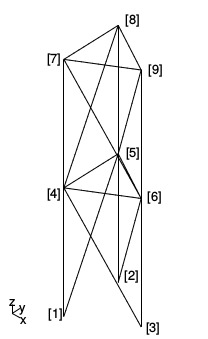
\includegraphics[height=0.3\textwidth]{images/finite_element.png}
  \caption{Finite element model, from \cite{peeters2000system}}
  \label{finite_el}
\end{figure}


\subsection{Continous-time state-space model} %(model parameters and reduction):

From the Equation (\ref{fondamental}) and with the variable change $x =
\begin{pmatrix}
\dot{q} \\
q
\end{pmatrix}$, we obtain the state equation:
\begin{equation}
\dot{x}(t) = A_cx(t) + B_cf(t)
\end{equation}
 where
$A_c =
\begin{pmatrix}
0 & I \\
M^{-1}K & M^{-1}C
\end{pmatrix}$
and
$B_c=
\begin{pmatrix}
0 \\
M^{-1}
\end{pmatrix}$

In a practical vibration experiment, not all $n$ degrees of freedom of the structure are measured, but only
a subset. The observation equation is:
\begin{equation}
y(t) = C_cx(t) + D_cf(t)
\end{equation}

If it is assumed that all $n$ degrees of freedom are measured and that the sensors are accelerometers transducers, we have
$C_c =
\begin{pmatrix}
M^{-1}K & M^{-1}C
\end{pmatrix}$
and
$D_c=
\begin{pmatrix}
M^{-1}
\end{pmatrix}$

Thus, the classical continuous-time state-space model is:
\begin{equation}
\left\{
\begin{array}{ll}
\dot{x}(t) = A_cx(t) + B_cf(t) \\
y(t) = C_cx(t) + D_cf(t)
\end{array}
\right.
\end{equation}

\subsection{Discrete-time state-space model} %(impulses response)

Up to now all equations were expressed in continuous time, whereas in reality
measurements are taken at discrete time instants.
So this model need to be converted to discrete time.
Another reason is that it is needed for performing simulations.

Thus, we choose a certain fixed sampling period $\Delta t$, and the continuous-time equations are discretized and solved at all
discrete time instants $k$ with $t = k \Delta t, k \in \mathbb{N}$.

The discrete-time state-space model is:
\begin{equation}
\left\{
\begin{array}{ll}
x_{k+1} & = A_dx_k + B_df_k \\
y_k & = C_dx_k + B_df_k
\end{array}
\right.
\label{discrete}
\end{equation}
where
\begin{equation}
\begin{array}{ll}
A_d = exp(A_c \Delta t) \\
B_d= (A_d - I) A^{-1}_c B_c \\
C_d = C_c \\
D_d = D_c
\end{array}
\end{equation}



%Stockastic state-space models
%ARMA models
%Continuous time frequency-domain models
%Discrete time frequency-domain models


\section{Localization using FRF interpolation method}


This method is presented in \cite{dilena2015damage}.
The main hypothesis underlying the method is that a concentrated damage reflects in a loss of spatial regularity of the
vibrational profile of a structure, compared with the reference (undamaged) state.

In this section, we suppose that we have $n$ sensors, which are located along an axis $z$, and we denote them by
$\{z_l\}, l\in \{1 ... n\}$. We also suppose we have $N$ measurements for each sensor.

For each sensor, we calculate the Frequency Response Function (FRF) from the acceleration's measures, at certain frequencies 
(which are $\frac{k}{N}, k \in \{0 ... N-1\}$).

Thus, for each frequency and each sensor, we have the transfer function value. Let us denote $H_R(z_l,f_i)$ the value of the transfer function for  the sensor $z_l$ at the frequency $f_i$.

Then, we calculate for each sensor $z_l$ the cubic polynomial spline interpolation of the transfer functions $H_R(z_k,f_i)$ measured at all 
the other instrumented locations $\{z_k\}, k\in \{1 ... n\}, k \neq l$: we denote it $H_S(z_l,f_i)$.

For these two transfer functions, we define the interpolation error $E(z_l,f_i)$ as the absolute value of the difference between recorded and interpolated FRFs:
\begin{equation}
E(z_l,f_i) = | H_R(z_l,f_i) - H_S(z_l,f_i) |
\end{equation}


\begin{figure}
  \centering
  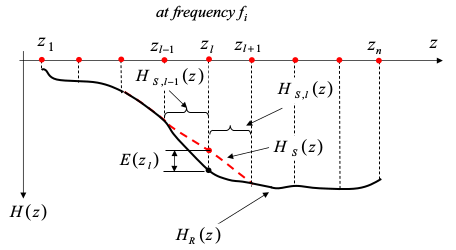
\includegraphics[width=0.4\textwidth]{images/interpolation.png}
  \caption{Interpolation error, from \cite{dilena2015damage}}
  \label{interpolation_error}
\end{figure}


Since we want to characterize each location $z_l$ with a scalar-valued error index, we introduce the norm of the error on the whole range of
frequencies:
\begin{equation}
E(z_l) = \sqrt{  \sum\limits_{i=1}^N  E^2(z_l,f_i) }
\label{error}
\end{equation}


Transfer function values obviously depend on the state of the structure. Hence, if the estimation of the error function
through Equation (\ref{error}) is repeated in the baseline (undamaged) and in the inspection (possibly damaged) configuration, then the
difference between the two values, denoted respectively by $E_0(z_l)$ and $E_d(z_l)$, can provide an indication about the existence of
degradation at location $z_l$:
\begin{equation}
\Delta E(z_l) = E_d(z_l) - E_0(z_l)
\end{equation}

An increase in the interpolation error between the reference configuration and the current configuration at a station $z_l$ , i.e.
$ \Delta E(z_l) > 0$, highlights a localized reduction of smoothness in the vibrational amplitude profile and, therefore, it is assumed
to be a symptom of a local variation of stiffness at $z_l$ associated with the occurrence of damage.

The above analysis has been developed in a deterministic context. Several sources, such as temperature, nonlinear
behavior, soil structure interaction and noise in recorded data, can induce variations of the interpolation error even if no
damage occurs.

Thus, once have to determine a threshold $E_T$, such as $ \Delta E(z_l)$ must be taller than $E_T$ to have a high probability of identification of a damage at location $z_l$. Indeed, as we can see in the Figure (\ref{proba}), the curves which represent the fact to have a damage or not have a share area: if the interpolation error $ \Delta E(z_l)$ is in this area, one can commit two errors:
\begin{itemize}
\item if it is in the area $P_f(z_l)$ under the graph of $p_{E,0}(z_l)$, once can detect a damage since there isn't one (false alarm).
\item if it is in the area $P_m(z_l)$ under the graph of $p_{E,d}(z_l)$, once can not detect a damage since there is one (missing alarm).
\end{itemize}


\begin{figure}
  \centering
  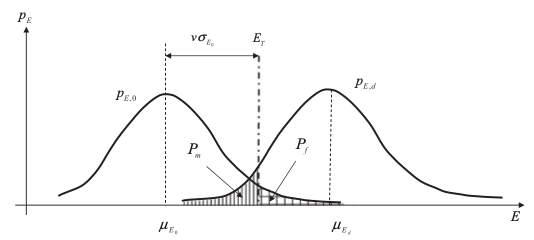
\includegraphics[width=0.4\textwidth]{images/gaussiennes.png}
  \caption{Probabilities of false and missing alarm, from \cite{dilena2015damage}}
  \label{proba}
\end{figure}


A detailled analysis of the statistical behaviour of the interpolation error is envisaged in the second part of this project.

\section{Simulation}

\subsection{Obtaining acceleration measures}

We have implemented a simulation to check this method of localization. We made this on the following system: $n$ masses, connected
through springs and dampers. We denote the masses $\{m_i\}_{i=1}^n$, the springs stifness $\{k_i\}_{i=1}^n$ and the dampers $\{c_i\}_{i=1}^n$ (see Figure (\ref{springs})).

\begin{figure}
  \centering
  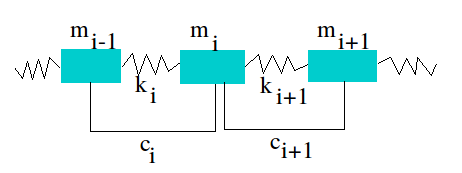
\includegraphics[width=0.4\textwidth]{images/ressorts.png}
  \caption{Masses connected through springs and dampers}
  \label{springs}
\end{figure}

For the simulation, we use the discrete-time state-space model (Equation (\ref{discrete})). First, we needed the matrices $M, C, K$. In this case, the matrices $M$ and $K$ are given by:
\begin{equation}
\begin{array}{l}
M = 
\begin{pmatrix} 
m_1\\ 
&\ddots\\ 
&&m_n
\end{pmatrix} 
\\
K = 
\begin{pmatrix} 
k_1 + k_2 & - k_1 \\ 
- k_1 &\ddots\\ 
& -k_i & k_i + k_{i+1} & -k_{i+1} \\
&&&\ddots& -k_n\\
&&& -k_n & k_n
\end{pmatrix} 
\end{array}
\end{equation}


Due to the lack of identifiable or measurable material
constants that govern the global damping behaviour of a structure, it is generally
impossible to assemble the damping matrix C in the same way as M and K.
Thus, we do the same thing that in practical situations: we consider that we are in the case of Rayleigh, i.e. a linear combination of the mass and stiffness matrix:
\begin{equation}
C = \alpha M + \beta K,\ \ \ \ \ \alpha, \beta \in \mathbb{R}_+
\end{equation}

With this matrices, we can calculate the matrices $A_c, B_c, C_c$ and $D_c$. To calculate the matrices $A, B$, we have to know the 
sampling period $\Delta t$. We need the frequencies of the system, because we have to respect the Nyquist–Shannon sampling theorem.
To determine the Nyquist frequency (here, it is the taller frequency of the system), we calculate the eigenvalues of $A_c$. Indeed, we have the link between the eigenvalues $\{\lambda_i\}_{i=1}^n$ and the frequencies of the system $\{f_i\}_{i=1}^n$:
\begin{equation}
\lambda_i = - \omega_i \xi_i \pm i \omega_i \sqrt{1 - \xi_i^2}
\end{equation}
where $\omega_i = 2 \pi f_i$ and $\xi_i$ is the damping ratio.

\begin{remark}
We can see that:\\
$|\lambda_i| = \sqrt{\omega_i^2 \xi_i^2 + \omega_i^2 (1 - \xi_i^2)} = \omega_i$
\end{remark}

\begin{remark}
The matrix $A_c$ has $2 \times n$ eigenvalues, but we obtain $n$ frequencies (for each eigenvalues, another one is its conjugated complex). 
\end{remark}

Now, we have the sampling period:
\begin{equation}
\Delta t = 2 \times max_{i \in \{1 ... n\} } f_i
\end{equation}

So we can calculate the matrices $A, B$ and make the simulation with the discrete-time state-space model (Equation (\ref{discrete})). To simulate the forces $f_k$, we use a white noise.

\subsection{Frequency Response Function}

The FRF correspond to the transfer function of the system. In frequency domain, if $F$ is the force that is apply on the system and $S$ is the response of this force, the FRF is given by:
\begin{equation}
H = \frac{S}{F}
\end{equation} 

We want to calculate the FRF of the system, for each sensor localization. Here, we calculate an estimation of the FRF, called $H_1$ estimator \cite{cauberghe2004applied}. We suppose we have a vector of the forces $\{ f_k\}_{k=1}^N$ and a vector of the accelerations $\{ y_k\}_{k=1}^N$ for each sensor (the two vectors are size $N$). We need to be in frequency domain, so we calculate the discrete Fourier transform:
\begin{equation}
\begin{array}{ll}
F_n = \sum\limits_{k=1}^N f_k e^{-2i\pi kn/N} \ \ \ \ \ n \in \{1 ... N\} \\
Y_n = \sum\limits_{k=1}^N y_k e^{-2i\pi kn/N} \ \ \ \ \ n \in \{1 ... N\}
\end{array}
\end{equation}

Then we calculate the power spectra, i.e. the Auto Power spectra of the inputs and the outputs
and the Cross Power spectra between the inputs and outputs respectively given by:

\begin{equation}
\begin{array}{ll}
S_{ff}(n) = F_n F_n^H \ \ \ \ \ n \in \{1 ... N\} \\
S_{yf}(n) = Y_n F_n^H \ \ \ \ \ n \in \{1 ... N\}
\end{array}
\end{equation}
where $M^H$ is the Hermitian of the matrix $M$. Thus, the FRF is given by:
\begin{equation}
H_1(n) = S_{yf}(n) S_{ff}(n)^{-1}
\end{equation}

\begin{remark}
If we consider each sensor separately, $F_n$ and $Y_n$ are scalars, so we have:
\begin{equation}
\begin{array}{lll}
H_1(n) & = & S_{yf}(n) S_{ff}(n)^{-1} \\
& = & Y_n F_n^H (F_n F_n^H)^{-1} \\
& = & Y_n / F_n
\end{array}
\end{equation}
\end{remark}

\subsection{Interpolation}

We have to calculate for each sensor $z_l$ and for each considered frequency $f_i$ the cubic polynomial spline interpolation of the transfer function $H_R(z_k,f_i)$.
The cubic spline interpolation is a piecewise continuous curve, passing through each of the values.
There is a separate cubic polynomial interpolation for each interval, each with its own coefficients.
Cubic polynomial spline interpolations produce an interpolated function that is continuous through to the second derivative.

With this interpolation, we can calculate the error as it is described in the section IV.

\subsection{Result}

For the simulation, we put a sensor on each mass.

Figure (\ref{frf_freq}) presents results of the FRF on the simulation datas: here is the curve of the FRF (absolute value) of one sensor (4 in total), in function of frequencies. We can see three peaks which are at the natural frequencies of the system, but there is one of these frequencies which not present a peak. Seeing this curve for each sensor, we observed that certain sensors have one peak for each natural frequencies, and others sensors have one peak for each except one, relied on the position of the sensor in the system. It is problematic because it is around the natural frequencies of the system that we have better datas, but if certain sensors haven't response with certain frequencies, we could miss out on a damage.


\begin{figure}
  \centering
  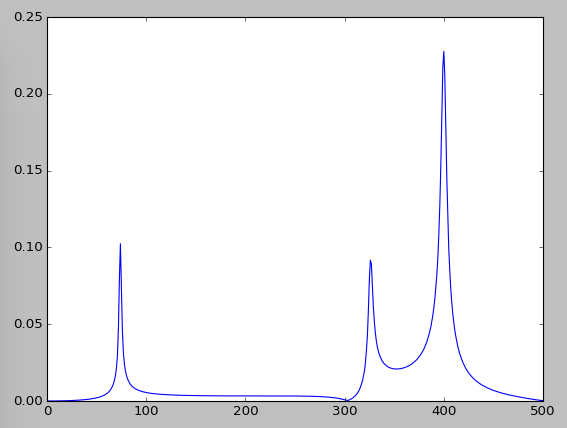
\includegraphics[width=0.3\textwidth]{images/FRF_freq.png}
  \caption{FRF of one sensor (4 in total), in function of frequencies}
  \label{frf_freq}
\end{figure}


Figure (\ref{damage}) is the FRF values for ten sensors (at a fixed frequency). Here, we easily can see that there is a damage between the sensors 4 and 5 (as we noticed it in the simulation).

\begin{figure}
  \centering
  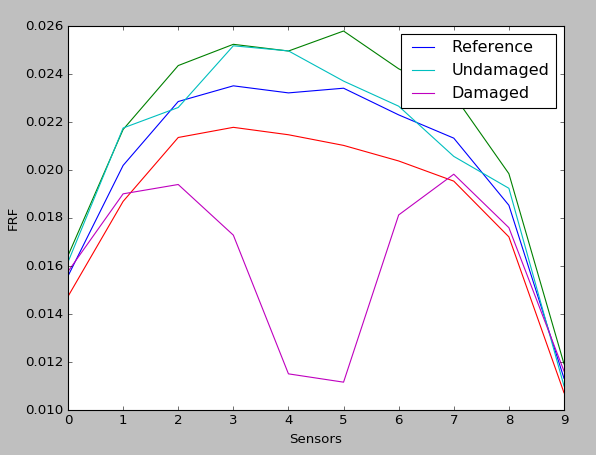
\includegraphics[width=0.3\textwidth]{images/curve_damage.png}
  \caption{FRF values for 10 sensors, at a fixed frequency}
  \label{damage}
\end{figure}


\section{Conclusion}




%\appendices
%\section{One appendix}
%some text for the appendix.

% use section* for acknowledgement
%\section*{Acknowledgment}
%The authors would like to thank...


%\begin{thebibliography}{1}
%
%\bibitem{IEEEhowto:kopka}
%H.~Kopka and P.~W. Daly, \emph{A Guide to \LaTeX}, 3rd~ed.\hskip 1em plus
%  0.5em minus 0.4em\relax Harlow, England: Addison-Wesley, 1999.
%
%\end{thebibliography}

\nocite{*}
\printbibliography

\end{document}



